% !TeX spellcheck = en_GB
% !TeX root = ../DistributedConsensus.tex
\chapter{Representing a History}\label{chap:representing-a-history}
	This chapter defines the representation of a History. Furthermore it examines why a local history of a single event must be totally ordered.
	
	\newpar	In a DCR graph where an event has been executed an arbitrary number of times, it is wanted to find the order of execution for the workflow. In order to find this, one must first determine how to represent an execution.
	
	\newpar An execution of an event leads to a set of changes in the workflow. These changes happen based on the relations that the workflow states. For the changes to happen the event must effect other events in certain ways. Furthermore since executions can happen multiple times, an execution also exists at a certain point in time, and so does every effect. This leads to the first definition of an execution:
	
	\begin{definition}
		An \textbf{execution} of an event can be represented as a finite set of effects, and their timestamps. The set of effects are determined by the workflow rules.
	\end{definition}
	
	Timestamps based on system clocks in distributed systems are not always synchronized, as described in \autoref{subsec:orderingofevents}, and therefore Lamport's logical clocks can be used for timestamps. Since an effect both has an event which performs the effect and another event which gets affected, we say that each effect has a counterpart:
	
	\todo[inline]{Ref. paper from Søren, located at \url{http://link.springer.com/chapter/10.1007\%2F978-3-319-19249-9_10}}

	\begin{definition}
		In a given effect where two events A and B are part of the effect, event B is \textbf{\textit{Counterpart}} of event A and event A is counterpart of event B.
	\end{definition}
	
	\newpar To be able to determine which event is performing the effect and which is the counterpart, it is necessary to use the ids of both. Furthermore to distinguish effects from eachother an effect type is necessary. Since an execution can happen multiple times and therefore affect the same counterpart multiple times, the counterpart timestamp is also necessary to distinguish different effects on the counterpart from each other. To distinguish multiple executions from each other an execution must have a start time and end time.
	
	\newpar For an event to know that something has happened it is neccesary to store it for later retrieval. This must be done not only for all the effects which happen in an execution but also when the event gets affected by another event.
	
	\newpar The representation of an effect has been named \textit{\textbf{Action}} because it can be seen as an action performed by an event in the DCR graph. An \textit{\textbf{Action}} is defined as:
	
	\begin{definition}
		An \textit{\textbf{Action}} consists of the ID of an event, the time stamp of the action, the ID and timestamp of a counterpart, as well as the type of the action.
	\end{definition}
	
	\newpar	The type of an effect is defined as an \textit{\textbf{Action Type}}:
	
	\begin{definition}
        \label{def:actiontype}
		An \textit{\textbf{Action Type}} can be one of the following:
		\begin{multicols}{3}
			\begin{enumerate}
				\item Includes\label{actiontype:includes}
				\item Included by\label{actiontype:includedby}
				\item Excludes\label{actiontype:excludes}
				\item Excluded by\label{actiontype:excludedby}
				\item Sets pending\label{actiontype:setspending}
				\item Set pending by\label{actiontype:setpendingby}
				\item Checks condition\label{actiontype:checkscondition}
				\item Checked condition by\label{actiontype:checkedconditionby}
				\item Execute start
				\item Execute finish
			\end{enumerate}
		\end{multicols}
	\end{definition}
	
	\newpar The action types 1 through 8 are related to the functionality of DCR graphs, i.e. \textit{Includes} is an action that happens when an event $A$ includes event $B$, similarly \textit{Included by} is an action that happens on event $A$ when event $B$ includes it. Action types 9 and 10 are action types that happen when an event starts executing and finishes executing. 
    
    \newpar
    An Action is part of an execution if the Event ID is the same and it has happened between a pair of \textit{Execute start} and \textit{Execute finish} actions. Furthermore, when an execution has an outgoing action the corresponding ingoing action is part of the execution as well, as illustrated in \autoref{fig:representing:execution} This is explained in \autoref{chap:order-of-execution}.
    
    \begin{figure}[H]
		\centering
		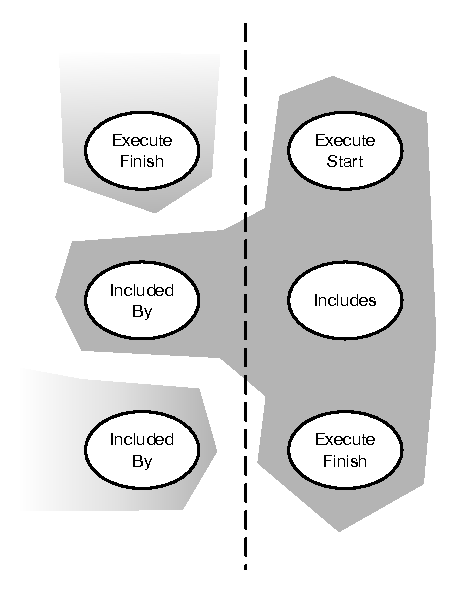
\includegraphics[height=\textheight/4]{3local/images/execution.pdf}
		\caption{Actions that are part of an execution across the history of two events.}
		\label{fig:representing:execution}
	\end{figure}\todo[inline]{Pilene på denne figur bør ikke være der, da vi stadig ikke har sagt noget om rækkefølgen på historikker. (Evt. lav en ny figur, og gem denne, da den nok kan bruges et andet sted)}
    
	With these new informations the definition of a representation of an exeuction can be revised to:
	
	\begin{definition}
		An \textbf{execution} of an event can be represented as a finite set of actions.
	\end{definition}
	
	\newpar Now that a representation of an execution and it's actions has been defined, it is necessary to define a way to connect and order these actions.
    
    \newpar When looking solely at the actions of a single event, we can compare each action with any other action and see which happened first by comparing their timestamps. For an action to be part of an execution, it has to happen after an \textit{Execute start} and before an \textit{Execute finish}.\todo[inline]{Skal vi komme nærmere ind på udefrakommende relationer, når afsnittet nu ikke længere er begrænset til et single-event-workflow?} Due to the requirement of DCR graphs that executions in an implementation must happen in a serially equivalent manner, all actions in execution A must either happen before or after all actions in execution B. This can be defined mathematically as follows when actions are compared on their logical timestamps:
	
	%\begin{center}
	%	$\forall_{x \in E_A}\forall_{y \in E_B} . (x < y) \lor \forall_{x \in E_A}\forall_{y \in E_B} . (y < x)$ \todo[inline]{Totality for executions?}
	%\end{center}

	\begin{center}
		$max_{E_A} < min_{E_B} \lor max_{E_B} < min_{E_A}$
	\end{center}
    
	\newpar Due to this property, executions happening on the same event are in  \textit{strict total order}. A strict total order can be represented as a list, but this is unfortunately not the case when the problem is extended with multiple events. Recall that Lamport states that it is not always possible to establish a strict total order of events in a distributed system, as described in \autoref{subsec:orderingofevents} - \nameref{subsec:orderingofevents}.\todo[inline]{Mikael: Personligt har jeg ikke behov for også at have navnet på afsnittet igen. Ved ikke med jer.}
	
    \begin{center}
    	\label{math:distributedExecutionOrder}
		$\forall_{x \in E_A}\forall_{y \in E_B} . ((x \rightarrow y \lor x \not\rightarrow y) \land y \not\rightarrow x)$
        
        $\lor$
        
        $\forall_{x \in E_A}\forall_{y \in E_B} . ((y \rightarrow x \lor y \not\rightarrow x) \land x \not\rightarrow y)$
        
        $\lor$
        
        $\forall_{x \in E_A}\forall_{y \in E_B} . (x \not\rightarrow y \land y \not\rightarrow x)$
	\end{center}
    \todo[inline]{Fiks Søren's kommentar: "I don't get this. What are you trying to show?"}\figuretodo{Mikael: Jeg tror det er nemmere at vise visuelt. Man kunne fx have en figur med to events, hvor event A kontakter event B, men event B afslutter en execution lige før den er kontaktet, og starter en ny lige efter. På to figurer er det så muligt at farvelægge de events der sker concurrently, før og efter event B's executions.}
    
	\newpar One can easily argue that a strict partial order fits ordering of actions because:
	\begin{enumerate}
		\item An action $A$ cannot happen before itself, therefore the order must be irreflexive.
		\item Actions $A$ and $B$, cannot both be happening before and after each other, therefore the order must be anti-symmetric.
		\item If action $A$ happened before action $B$ and $B$ happened before $C$ then $A$ happened before $C$ and the order must be therefore transitive.
		\item Actions can in distributed systems be concurrent and the order can therefore not be total.
	\end{enumerate}
	\newpar Since a finite strict order can be represented as a directed acyclic graph the history can therefore also be represented as such, where actions are nodes and the order in which the actions have happened is represented as edges.
	%\begin{enumerate}
	%	\item Actions can be represented as nodes in the graph. The ordering of actions can be represented as the edges between the nodes.
	%	\item Paths from one action to another can be found by going over edges. Finding these paths explain which transitive relations each action has.
	%	\item A graph can represent concurrent actions by having two nodes A and B, where there exists no path from A to B and from B to A.
	%	\item The acyclic requirement ensure that action A cannot occur both before and after action B since there is no path from both A and B and from B to A.
	%	\item The acyclic requirement also ensures that action A cannot have an edge to itself, implying that it happened before itself.
	%\end{enumerate}
	
	\newpar This leads to the following definition of \texttt{History}:
	
	\begin{definition}
		A \textit{\textbf{History}} is a strict partial order of actions.
	\end{definition}
	
    \newpar 
    A \textit{global history} is the strict partial order of the actions of all events in the workflow. A \textit{local history} is a strict total order of the actions that have happened on a single event. \todo[inline]{Kan definitionen og den efterfølgende tekst ikke komme før vi nævner det med DAC?}
	
%	\begin{figure}
%		\centering
%		\import{3local/images/}{singleexecution.pdf_tex}
%		\caption{History representation of a single execution of the Event \texttt{ReadGasMeter}.}
%		\label{fig:local:readgasmeterhistory}
%	\end{figure}

%	\newpar When creating a history from the local database, the actions are added as nodes in the history, and since the ordering is total we can add edges between consecutive actions. An example of a local history is shown in \autoref{fig:local:readgasmeterhistory}.
	
	
%	\newpar In the implementation, we have created two types representing an action. One, the \texttt{ActionModel} is used for storage in the ORM Entity Framework.\footnote{Object-Relational Mapping, used for mapping between objects in an object-oriented paradigm and relations in a relational database.}\footnote{\url{https://msdn.microsoft.com/en-us/data/ef.aspx}} As this mapping is set up in a C\# library, this had to be a C\# class as well. The \texttt{ActionModel} uses the enum \texttt{ActionType} to denote the action type.
%	
%	The other type is created in the F\# module \texttt{HistoryConsensus} that contains most of the program described throughout this report. The \texttt{ActionType} in this module is a discriminated union, where each case represents a single type.\footnote{\url{https://msdn.microsoft.com/en-us/library/dd233226.aspx}}
%	In this module the type \texttt{ActionId} is defined as a tuple of an event ID and a local timestamp. The \texttt{Action} is then defined as a record  with two \texttt{ActionId}s, a local and a counterpart, as well as an \texttt{ActionType}.
%	
%	The \texttt{History} is implemented as a record with a single label called \texttt{Nodes}, containing a \texttt{Map} mapping from \texttt{ActionId} to the \texttt{Action} itself.
%	
%	\newpar As everything is handled locally at the event, no messages are passed between computers, other than the initial request for the local history, as well as the response. Retrieval of data from the database, as well as building the totally ordered history, takes time linear in the number of actions for that event, since the database is sorted and each event is accessed and used one at a time only once.
%	
%	\newpar In the case where a single event creates history, the event contacted has to be trusted as not being malicious. If the event cannot be trusted as behaving correctly, there are no guarantees that the history is correct, as it is the only source of its local history. Handling malicious nodes will be discussed further in the following chapters.
